\documentclass[a4paper,11pt,twocolumn]{article}
\usepackage[latin1]{inputenc}
\usepackage[english]{babel}
\usepackage{amsmath}
\usepackage{amsfonts}
\usepackage{amssymb}
\usepackage{cuted}

\usepackage{titling}
\usepackage{nomencl}
\usepackage{siunitx}
\usepackage[style=ieee,backend=bibtex]{biblatex}
\usepackage[font={small}]{caption}

\usepackage{graphicx}
\usepackage{color}

\usepackage{booktabs}
\usepackage{threeparttable}
\usepackage{fancyhdr}
\usepackage{float}

\usepackage{varioref}
\usepackage{textcomp}
\usepackage{xspace}
\usepackage[activate={true,nocompatibility},final,tracking=true,kerning=true,spacing=nonfrench,factor=1100,stretch=10,shrink=10]{microtype}
% activate={true,nocompatibility} - activate protrusion and expansion
% final - enable microtype; use "draft" to disable
% tracking=true, kerning=true, spacing=true - activate these techniques
% factor=1100 - add 10% to the protrusion amount (default is 1000)
% stretch=10, shrink=10 - reduce stretchability/shrinkability (default is 20/20)

% Reduce tracking around small caps to 40%
\SetTracking{encoding={*}, shape=sc}{40}
\newcommand{\Textregistered}{\textsuperscript{\textregistered}\xspace}
\newcommand{\Texttrademark}{\texttrademark\xspace}

\newcommand{\s}{\si{\second}\xspace}
\newcommand{\W}{\si{\watt}\xspace}
\newcommand{\V}{\si{\volt}\xspace}
\newcommand{\A}{\si{\ampere}\xspace}
\newcommand{\Ohm}{\si{\ohm}\xspace}
\renewcommand{\H}{\si{\henry}\xspace}
\newcommand{\mH}{\si{\milli\henry}\xspace}
\newcommand{\Nm}{\si{\newton\metre}\xspace}
\newcommand{\rps}{\si{\radian\per\second}\xspace}
\newcommand{\Vspr}{\si{\volt\second\per\radian}\xspace}
\newcommand{\NmpA}{\si{\newton\metre\per\ampere}\xspace}
\newcommand{\kgmm}{\si{\kilogram\square\metre}\xspace}
\newcommand{\Nmspr}{\si{\newton\metre\second\per\radian}\xspace}
\newcommand{\RPM}{\text{RPM}\xspace}

\newcommand{\AC}{a.c.\xspace}
\newcommand{\DC}{d.c.\xspace}
\newcommand{\EMF}{e.m.f.\xspace}
\newcommand{\TRBDFII}{\textsc{tr-bdf\footnotesize2}\xspace}
\newcommand{\odetwothreebt}{ode\oldstylenums{23}bt\xspace}
\newcommand{\SW}[1]{\textsc{sw\footnotesize#1}\xspace}

% Document info.
\author{Z0966990}
\title{E27 Lab Report}
\date{\today}

% Path to images.
\graphicspath{{img/}}

% Setup nomenclature.
\newlength{\nomtitlesep}
\setlength{\nomtitlesep}{\nomitemsep}
\setlength{\nomitemsep}{-\parsep}
\renewcommand\nomgroup[1]{
    \ifthenelse{\equal{#1}{A}}{
        \itemsep\nomtitlesep
        \item[\textbf{Acronyms}]
        \itemsep\nomitemsep}{
    \ifthenelse{\equal{#1}{B}}{
        \itemsep\nomtitlesep
        \item[\textbf{Variables}]
        \itemsep\nomitemsep}{
}}}
\newcommand{\nomindex}[1]{
    \hspace*{\fill}
    \makebox[5em][l]{#1}
}
\makenomenclature

% Setup bibiliography.
\addbibresource{bibliography}

% Header and footer.
\pagestyle{fancy}
\fancyhf{}
\lhead{\thetitle}
\rhead{\theauthor}
\cfoot{\thepage}
\renewcommand{\headrulewidth}{0pt}
\renewcommand{\footrulewidth}{0pt}

\begin{document}
    
% Title page.
\begin{titlepage}
    \centering
    \vspace*{\fill}
    
\includegraphics[width=0.5\textwidth]{Durham}\\
    \vspace*{\fill}
    \LARGE\thetitle\\
    \large\theauthor\\
    \large L2 Electrical Engineering\\
    \large\thedate\\
    \vspace*{\fill}
\end{titlepage}

% Main matter.
\renewcommand{\abstractname}{\large Abstract}
\twocolumn[
\begin{@twocolumnfalse}
    \begin{abstract}
        In this report, it is described how the MathWorks\Textregistered 
        Simulink\Textregistered and SimScape\Texttrademark graphical packages 
        were used to model the way electrical and mechanical properties of a 
        separately excited \DC motor changed with respect to time. Using 
        results from the simulation and the torque error term, it was shown the 
        motor was capable of outputting enough torque to match the load at a 
        range of different speeds.
    \end{abstract}
\end{@twocolumnfalse}
\vspace{\parsep}
]

% Acronyms
\nomenclature[A0]{\AC}{Alternating current}
\nomenclature[A1]{\DC}{Direct current}
\nomenclature[A2]{\EMF}{Electromotive force}
\nomenclature[A3]{r.p.m.}{Revolutions per minute}

% Variables
\nomenclature[B00]{$B$}{Load torque constant \nomindex{\Nmspr}}
\nomenclature[B01]{$E$}{Motor back \EMF \nomindex{\V}}
\nomenclature[B02]{$I$}{Current \nomindex{\A}}
\nomenclature[B03]{$J$}{Moment of inertia \nomindex{\kgmm}}
\nomenclature[B04]{$K$}{Motor \EMF constant \nomindex{\NmpA}\\\nomindex{\Vspr}}
\nomenclature[B05]{$L$}{Inductance \nomindex{\H}}
\nomenclature[B06]{$N$}{Motor speed \nomindex{\RPM}}
\nomenclature[B08]{$R$}{Resistance \nomindex{\Ohm}}
\nomenclature[B09]{$T$}{Torque \nomindex{\Nm}}
\nomenclature[B10]{$V$}{Supply voltage \nomindex{\V}}
\nomenclature[B11]{$t$}{Time \nomindex{\s}}
\nomenclature[B12]{$\omega$}{Motor speed \nomindex{\rps}}
\nomenclature[BB]{}{\vspace{-1em}\nomindex{}}

\printnomenclature

\section{Introduction}

Direct current motors are used in a variety of applications from power tools to 
electric vehicles. Unlike alternating current motors, a \DC motor can be 
battery powered so are typically found in portable applications. However, 
precise torque and speed control is the primary benefit of \DC motors over 
their \AC counterparts. Motors driven by an alternating supply typically 
operate at a fixed frequency and speed, requiring \AC/\AC convertors to change 
the supply frequency \cite[p. 787]{hughes2010hughes}.

As detailed in the remainder of the report, the speed of \DC motors can be 
varied by changing the magnitude of the \DC supply voltage, provided the motor 
can meet the loading requirements.

\section{Background} \label{sec:Background}

According to Hughes in \cite[p.~870]{hughes2010hughes}, the most general form 
of \DC motor is a separately excited \DC motor, where the motor consists of two 
distinct parts---the stator field and armature---which each have their own 
independent \DC voltage source. Under constant field operation, the magnetic 
field produced by current flowing through the field windings is unchanging. As 
current flows through windings in the armature, an electric field is produced 
which interacts with the static magnetic field. This interaction exerts an 
electromagnetic torque $T_e$ on the armature, shown to be proportional to the 
armature current $I_a$ as follows \cite[p.~873]{hughes2010hughes}:

\begin{equation}  \label{eq:T}
    T_e = K I_a ~\Leftrightarrow~ I_a = \frac{T_e}{K} \\
\end{equation}

The motor \EMF constant relates electromagnetic torque to armature current and 
is composed of the field current $I_f$ and the coupling inductance between the 
field and stator windings $L_{af}$. According to \cite{brigham2016coursework}, 
it is defined by the following:
\begin{equation} \label{eq:K}
    K = L_{af} I_f \\
\end{equation}

Figure~\vref{fig:Circuit} contains the circuit diagram of a separately excited 
\DC motor subjected to a load torque $T_L$---based on the diagram given in 
\cite{kazemtabrizi2015dc}. When there is a net torque on the armature the motor 
accelerates to some non-zero rotational speed. Consequently, the armature 
current moves relative to the stator field, so a back \EMF is induced across 
the armature windings such that it opposes its supply voltage in accordance 
with Faraday and Lenz's laws. Hughes shows the same motor constant from 
Equation~\ref{eq:K} relates the back \EMF $E$ to the rotational speed $\omega$ 
\cite[p.~873]{hughes2010hughes}.
\begin{equation}  \label{eq:omega}
    E = K \omega ~\Leftrightarrow~ \omega = \frac{E}{K} \\
\end{equation}

\begin{figure}[h]
    \centering
    \def\svgwidth{0.48\textwidth}
    \input{img/Circuit.pdf_tex}
    \caption{Circuit diagram of a seperately excited \DC motor.}
    \label{fig:Circuit}
\end{figure}

During the initial phase of operation, the rotational speed of the armature is 
small. As a result---according to Equation~\ref{eq:omega}---the back \EMF is 
similarly small. As armature windings do not have a large resistance, this 
results in a potentially damaging current. To compensate, the starting 
resistance $R_{st}$ in  Figure~\ref{fig:Circuit} is set to some sufficiently 
large value to limit the current in the armature.

Applying Kirchoff's voltage law to the left hand side of 
Figure~\ref{fig:Circuit}, an equation linking all the electrical properties of 
the armature is found:
\begin{equation}  \label{eq:ERst}
    E = V - I_a(R_a + R_{st}) \\
\end{equation}

However, under normal operation after the motor has started, the resistance 
$R_{st}$ is taken out of the armature to achieve a greater electromagnetic 
torque. The following equation describes how the electrical properties of the 
armature are related under normal operation and is the equation given by Hughes 
\cite[p.~871]{hughes2010hughes}:
\begin{equation}  \label{eq:E}
    R_{st} = 0~\Ohm ~\Rightarrow~ E = V - I_a R_a \\
\end{equation}

\section{Methods}

The Simulink package and SimScape library produced by MathWorks were used to 
model the behaviour of a \DC motor system with a two step motor starter---using 
an implementation of \TRBDFII developed in \cite{bank1985transient, 
hosea1996analysis}. In Simulink, \TRBDFII is used in the \odetwothreebt solving 
method. The block diagram of the model the solver was used on is documented in 
Figure~\vref{fig:Model}. 
\begin{figure*}[t]
    \centering
    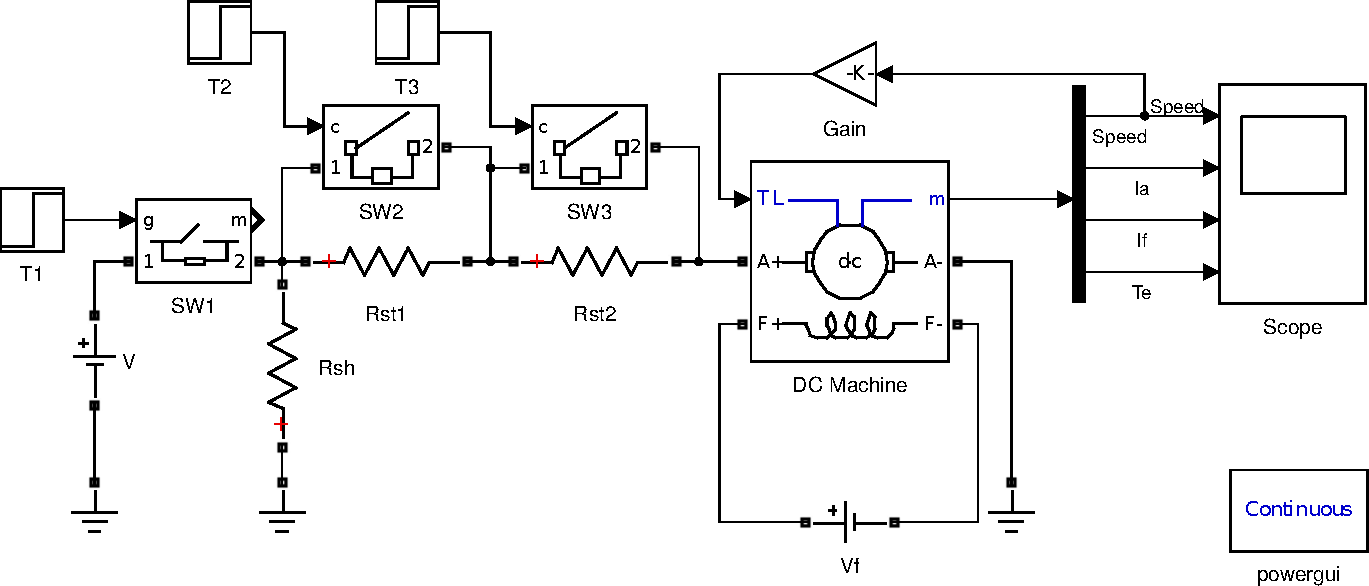
\includegraphics[width=\textwidth]{Model}
    \caption{Block diagram of the Simulink model.}
    \label{fig:Model}
\end{figure*}

The \DC machine was configured with the moment of inertia, resistance and 
inductance of the armature and field windings given in 
Table~\vref{table:Parameters}. The electrical inputs for these windings were 
implemented using external \DC voltage sources; the magnitudes of which were 
also given in Table~\ref{table:Parameters}. For monitoring purposes, the output 
signals of the motor were armature current, field current, electromagnetic 
torque and speed.
\begin{table}[h]
    \centering
    \footnotesize
    \begin{threeparttable}
        \caption{Defining parameters of \DC motor system.\vspace{-\parsep}}
        \label{table:Parameters}
        \begin{tabular}{@{}llrl@{}}
            \toprule
            \multicolumn{4}{l}{\textbf{Armature Components}} \\
            \hspace{1em}$V$   & Supply voltage      & 240 & \V \\
            \hspace{1em}$R_a$ & Armature resistance & 1.6 & \Ohm \\
            \hspace{1em}$L_a$ & Armature inductance &  12 & \mH \\
            \hspace{1em}$J$   & Moment of inertia   & 0.5 & \kgmm \\
            \midrule
            \multicolumn{4}{l}{\textbf{Field Components}} \\
            \hspace{1em}$V_f$    & Field voltage       &  240 & \V \\
            \hspace{1em}$R_a$    & Field resistance    &  240 & \Ohm \\
            \hspace{1em}$L_a$    & Field inductance    &  120 & \H \\
            \hspace{1em}$L_{af}$ & Coupling inductance & 1.65 & \H \\
            \midrule
            \multicolumn{4}{l}{\textbf{Load Characteristics}} \\
            \hspace{1em}$T_{e0}$   & Initial torque         & 45       & \Nm \\
            \hspace{1em}$\omega_0$ & Initial speed          &  1       & \rps \\
            \hspace{1em}$B$        & Load constant\tnote{*} & 0.247969 & \Nmspr 
            \\
            \bottomrule
        \end{tabular}
        \begin{tablenotes}
            \item[*]See Equation~\vref{eq:B}.
        \end{tablenotes}
    \end{threeparttable}
\end{table}

The \DC machine was also configured with a starting field current as this would 
be constant throughout the simulation. Applying Ohm's law to the right hand 
side of Figure~\ref{fig:Circuit}, the stable field current was found:
\begin{align*}
    I_f &= \frac{V_f}{R_f} \\
    I_f &= \frac{240~\V}{240~\Ohm} \\
    I_f &= 1~\A
\end{align*}

A constant useful for calculating additional model parameters was the motor 
\EMF constant; it's value was found by substituting the coupling inductance 
from Table~\ref{table:Parameters} and the constant field current into 
Equation~\ref{eq:K}. The calculation yielded the following result:
\begin{align*}
    K &= L_{af} I_f \\
    K &= (1.65~\H) (1~\A) \\
    K &= 1.65~\Vspr
\end{align*}

Using the motor \EMF constant, the theoretical armature current at nominal 
speed can be calculated. The nominal speed given in 
\cite{brigham2016coursework} was 1220~\RPM; this had to be converted into \rps:
\begin{equation*}
    N = 1220~\RPM~\Leftrightarrow~\omega = 122\pi/3~\rps
\end{equation*}

Equation~\ref{eq:omega} was substituted into Equation~\ref{eq:E} then 
rearranged to make $I_a$ the subject. The armature current at nominal speed was 
found by plugging in values from Table~\ref{table:Parameters} and the nominal 
speed calculated above, as follows:
\begin{align*}
    K \omega &= V - I_a R_a \\
    \Leftrightarrow~ I_a &= \frac{V - K \omega}{R_a} \\
    I_a =& \frac{240~\V - (1.65~\Vspr)(122\pi/3~\rps)}{1.5~\Ohm} \\
    I_a =& 19.466~\A
\end{align*}

\subsection{Electric Hoist Load}

The motor in the simulation was loaded with an electric hoist--type load. The 
rotational speed $\omega$ was used to described the load torque $T_L$ 
using the following relationship:
\begin{equation} \label{eq:B}
    T_L = B\omega \\
\end{equation}

This was modelled by connecting the speed output of the \DC machine to the 
torque load input via a constant gain block, configured with the multiplicative 
gain $B$ given in Table~\ref{table:Parameters}. The topology of the network can 
be seen in the top-right of Figure~\ref{fig:Model}.

\subsection{Motor Starter} \label{sec:MotorStarter}

The motor starter in this model---represented as a variable resistor in 
Figure~\ref{fig:Circuit}---was modelled using three switches in series with the 
armature winding. Two of the switches were parallel to a resistor, such that 
all current flowed through the resistor when the switch was open: when the 
switch was closed the current experienced no resistance. 
Figure~\vref{fig:Starter} shows the circuit diagram of the network implemented, 
with the switches open as they were at the start of the simulation.
\begin{figure}[h]
    \centering
    \def\svgwidth{0.48\textwidth}
    \input{img/Starter.pdf_tex}
    \caption{Circuit diagram of the motor starter used in the model.}
    \label{fig:Starter}
\end{figure}

An ideal switch was used to model \SW{1} and circuit breakers were used to 
model \SW{2} and \SW{3}. These were closed at 0.5~\s, 2.5~\s and 3.5~\s 
respectively using step blocks; this can be seen in Figure~\vref{fig:Model}. 
The 0.5~\s delay before powering the armature winding gave the field current 
and armature mechanics sufficient time to stabilise, whilst the other two 
switches removed the starting resistance in two steps.

The starting resistance limited the current flowing through the armature 
winding---to prevent damage---but the current had to be sufficiently large to 
generate the initial 45~\Nm of electromagnetic torque prescribed in 
Table~\ref{table:Parameters}.

The maximum allowable starting resistance $R_{st\,max}$ was calculated by 
substituting Equations~\ref{eq:K} and \ref{eq:omega} into 
Equation~\ref{eq:ERst} and rearranging for $R_{st}$. The initial speed of the 
armature was assumed to be 1~\rps. The result after substituting the necessary 
values was as follows:
\begin{align*}
    K \omega &= V - \frac{T_e}{K}(R_a + R_{st}) \\
    \Leftrightarrow~ R_{st} &= \frac{V - K\omega}{T_e/K} - R_a \\
    R_{st\,max} &= \frac{240~\V - (1.65~\Vspr)(1~\rps)}{(45~\Nm)/(1.65~\NmpA)}\\
        &\hspace{13em} - 1.5~\Ohm \\
    R_{st\,max} &= 7.2395~\Ohm
\end{align*}

Each of the resistors marked Rst1 and Rst2 in the Figure~\vref{fig:Model} were 
configured with half the maximum allowable starting resistance: 3.6197~\Ohm.

\subsection{Variable Speed Operation}

The simulation model was also used to test the effectiveness of varying the 
speed of the motor by reducing the supply voltage. The target nominal speed was 
800~\RPM, which first had to be converted into \rps before the new supply 
voltage could be found:
\begin{equation*}
    N = 800~\RPM~\Leftrightarrow~\omega = 80\pi/3~\rps
\end{equation*}

To achieve a speed of $80\pi/3~\rps$, the motor would have to match load torque 
exerted by the electric hoist. The load torque at this speed was found by 
substituting the speed in \rps into Equation~\vref{eq:B} as follows:
\begin{align*}
    T_L &= B\omega \\
    T_L &= (0.247969~\Nmspr)(80\pi/3~\rps) \\
    T_L &= 20.774~\Nm
\end{align*}

The armature current required to produce an equivalent amount of 
electromagnetic torque was found by substituting the load torque into 
Equation~\ref{eq:T}, as follows:
\begin{align*}
    I_a &= \frac{T_e}{K} \\
    I_a &= \frac{20.774~\Nm}{1.65~\NmpA} \\
    I_a &= 12.590~\A
\end{align*}

Finally, the required supply voltage was found by substituting 
Equation~\ref{eq:omega} into Equation~\ref{eq:E} and rearranging for $V$. The 
$R_{st}$ term could be neglected, as at nominal speed the motor should have 
already started and stabilised.
\begin{align*}
    K \omega &= V - I_a R_a \\
    \Leftrightarrow~V &= K \omega + I_a R_a \\
    V &= (1.65~\Vspr)(80\pi/3~\rps) \\
        &\hspace{6em}+ (12.590~\A)(1.5~\Ohm) \\
    V &= 157.12~\V
\end{align*}

The \DC voltage source for the armature winding was reconfigured with a
magnitude of 157.12~\V.

\section{Results and Discussion}

Figure~\vref{fig:Time240V} shows the evolution of the \DC machine parameters 
during the 5~\s simulation, performed at the original supply voltage of 240~\V.
Note the discontinuities at 0.5~\s, 2.5~\s and 3.5~\s; when \SW{1}, \SW{2} and
\SW{3} were closed.
\begin{figure*}[t]
    \centering
    \def\svgwidth{0.75\textwidth}
    \input{img/Time240V.pdf_tex}
    \caption{Simulated motor properties against time with 240~\V supply.}
    \label{fig:Time240V}
\end{figure*}

Those sudden increases in electromagnetic torque output can be attributed to 
the increases in armature current. Indeed, Equation~\ref{eq:T} showed 
electromagnetic torque is directly proportional to the armature current.

As discussed in Section~\ref{sec:MotorStarter}, when each of \SW{2} and \SW{3} 
were closed, the switch established a branch parallel with the resistor. The 
resistance of such a network is zero. Thus at 2.5~\s and 3.5~\s the starting 
resistance $R_{st}$ decreased. Rearranging Equation~\ref{eq:ERst} for $I_a$, it 
is clear the decrease in starting resistance was responsible for the sudden 
increase in armature current:
\begin{equation} \label{eq:Ia}
    I_a = \frac{V - E}{R_a + R_{st}}
\end{equation}

Equation~\ref{eq:Ia} also explains why the torque decayed soon after 
each switch was closed. The armature had a rotational inertia of 0.5~\kgmm, so 
the armature speed lagged the net torque; this was evidenced in 
Figure~\ref{fig:Time240V}---the rotational speed did not instantly change in 
reaction to the increase in electromagnetic torque. However, as the armature 
slowly accelerated, the back \EMF increased according to 
Equation~\ref{eq:omega}. The increasing back \EMF reduced the current flowing 
through the armature and thus the torque decayed.

As the armature speed increased, electromagnetic torque decreased, but the load 
torque increased linearly---see Equation~\ref{eq:B}. The net torque $T_e - T_L$ 
driving the acceleration of the armature became smaller as the armature reached 
higher speeds. In Figure~\ref{fig:Time240V} this is apparent as the rate of 
change of armature speed became smaller as time progressed. Ideally, the net 
torque would be zero at the nominal speed: $1220~\RPM = 122\pi/3~\rps = 
127.76~\rps$. Figure~\ref{fig:Time240V} suggests that by 5~\s, the motor had 
reached nominal speed.

Figure~\vref{fig:TorqueSpeed240V} is the torque--speed plot for the simulation. 
Inspection of the load and electromagnetic torque traces suggest the torques 
converged at the nominal speed of 127.76~\rps---the operating point where there 
was no net torque. The motor error term $\Delta T$ can be used to quantify the 
capability of the motor matching the full load torque at nominal speed. The 
error term is given by the following equation:
\begin{equation} \label{eq:DeltaT}
    \Delta T = \frac{T_e - T_L}{T_{L\,max}}
\end{equation}
\begin{figure*}[t]
    \centering
    \def\svgwidth{0.75\textwidth}
    \input{img/TorqueSpeed240V.pdf_tex}
    \caption{Torque--speed plot of simulation with 240~\V supply.}
    \label{fig:TorqueSpeed240V}
\end{figure*}

Where $T_e$ and $T_L$ were recorded at 5~\s and the full load torque 
$T_{L\,max}$ was calculated by substituting the nominal speed into 
Equation~\ref{eq:B}. From these values, the error term for the 1220~\RPM 
simulation was computed using Equation~\ref{eq:DeltaT} as follows:
\begin{align*}
    \Delta T &= \frac{T_e - T_L}{T_{L\,max}} \\
    \Delta T &= \frac{31.798~\Nm - 31.664~\Nm}{31.680~\Nm} \\
    \Delta T &= 0.42333\%
\end{align*}

Acceptable values for the error term are smaller than 1\%, and indicate the 
motor was capable of matching the full load torque to within an acceptable 
degree of error. As the error term for this simulation was 0.42333\%, the motor 
used in the simulation was successful at matching the full load torque. The 
error term was non-zero because the field winding inductance of 12~\mH, whilst 
small, was also non-zero. The current would require an infinite amount of time 
to converge on a value where the load torque and electromagnetic torque match, 
so in practical applications error terms of zero are impossible.
\begin{figure*}[t]
    \centering
    \def\svgwidth{0.75\textwidth}
    \input{img/TorqueSpeed157V.pdf_tex}
    \caption{Torque--speed plot of simulation with reduced 157.12~\V supply.}
    \label{fig:TorqueSpeed157V}
\end{figure*}

Figure~\vref{fig:TorqueSpeed157V} shows the torque--speed plot for the 
simulation after the supply voltage had been reduced to 157.12~\V in order to 
achieve a nominal speed of $800~\RPM = 80\pi/3~\rps = 83.776~\rps$. Examining 
Figure~\ref{fig:TorqueSpeed157V}, the load and electromagnetic torque appeared 
to converge at the nominal speed---the operating point; they converged in a 
similar manner to the torque--speed curves in Figure~\ref{fig:TorqueSpeed240V}.

The error term was calculated as before:
\begin{align*}
    \Delta T &= \frac{T_e - T_L}{T_{L\,max}} \\
    \Delta T &= \frac{20.817~\Nm - 20.723~\Nm}{20.774~\Nm} \\
    \Delta T &= 0.42249\%
\end{align*}

At the reduced speed, the motor was also capable of matching the full load 
torque to within an acceptable degree of error.

\section{Conclusion}

At low speeds, \DC motors are susceptible to armature damage due to large 
currents. Whilst the motor starter resistance system was successful in 
reducing the armature current while starting the motor, the armature current 
still reached its peak value when the motor was accelerating up to nominal 
speed.

Varying the armature supply voltage was an effective method of varying the 
nominal speed of the \DC motor. The motor used was capable of matching the 
target speeds of 1220~\RPM at 240~\V and 800~\RPM at 157.12~\V whilst meeting 
torque requirements of the electric hoist--type load specified to within an 
acceptable accuracy of 0.42333\% and 0.42249\% respectfully.

% References.
\printbibliography

\end{document}
